\documentclass{article}
\usepackage[utf8]{inputenc}

\title{Sistemas Inteligentes}
\author{Isabela Marinho Ribeiro }
\date{Novembro de 2019}

\usepackage{natbib}
\usepackage{graphicx}
\usepackage{indentfirst}





\begin{document}

\maketitle

\section{Introdução}
\label{drive}
\label{cadeira}
\label{arvore}
A disciplina de Sistemas Inteligentes é um subcampo na área de Inteligência Artificial dentro da Computação. \cite{drive} Nela, o aluno tem como objetivo treinar sistemas a reconhecer padrões através de uma grande quantidade de dados disponível. Por meio deles, um programa pode melhorar seu desempenho com a experiência. \cite{cadeira} Entre os principais tópicos que compõem a disciplina estão Árvores de Decisão e Redes Neurais. \cite{arvore} As Arvores de Decisão consistem em um método de aprendizado de máquina relativamente acessível, no qual os dados são divididos por meio de ramificações baseadas em variáveis. Já as Redes Neurais são conjuntos de sistemas que, com o uso de algoritmos, funcionam como neurônios que captam padrões escondidos e correlações entre dados, melhorando assim o desempenho na prática.

\begin{figure}[h!]
\centering
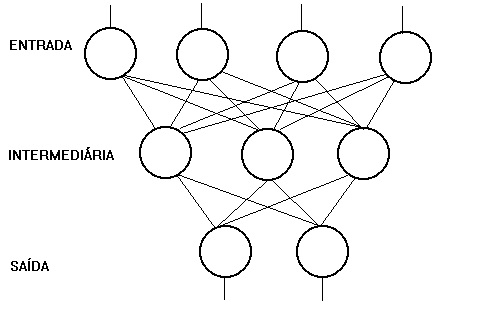
\includegraphics[scale=0.6]{redes.jpg}
\caption{\cite{1} Diagrama de uma Rede Neural}
\label{fig:redes.jpg}
\end{figure}

\section{Relevância}
A Inteligência Artificial é uma área da computação em crescimento constante e rápido, além de estar se popularizando cada vez mais no dia a dia, com assistentes pessoais, jogos eletrônicos e até em câmeras de segurança. Na disciplina de Sistemas Inteligentes, vê-se uma introdução teórica consistente ao assunto, além de aulas práticas que complementam o conhecimento.


\section{Relação com outras disciplinas}
\label{maquina}
Os tópicos principais da disciplina de Sistemas Inteligentes estão fortemente ligados às disciplinas de Aprendizagem de Máquina \cite{maquina} e Redes Neurais, as quais se aprofundam nos conceitos de Árvores de Decisões e de Redes Neurais como cadeiras eletivas.

\begin{figure}[h!]
\centering
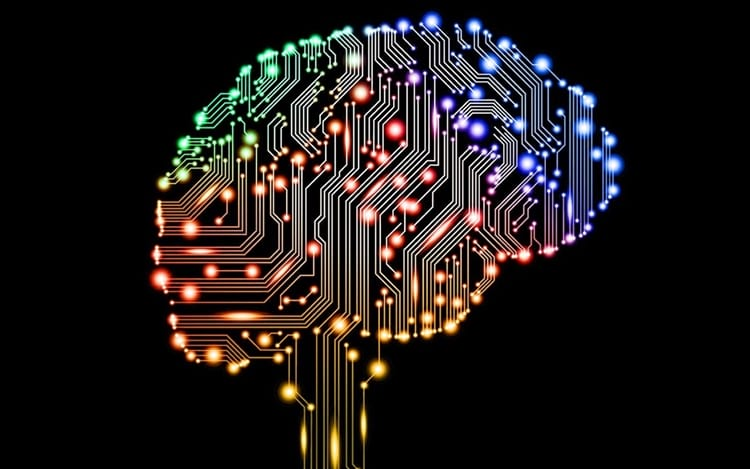
\includegraphics[scale=0.4]{cerebro.jpg}
\caption{\cite{2} Os algoritmos das redes neurais se baseiam nos neurônios do cérebro humano.}
\label{fig:cerebro.jpg}
\end{figure}


\bibliographystyle{plain}
\bibliography{imr}


\end{document}
